I sistemi di Machine Learning vengono generalmente sviluppati assumendo che i dati osservati durante l'addestramento siano rappresentativi di quelli che il modello incontrerà durante il suo utilizzo. Nelle applicazioni reali, tuttavia, questa assunzione è spesso disattesa: le caratteristiche della distribuzione dei dati possono variare nel tempo o tra differenti contesti di utilizzo. Questo fenomeno, comunemente indicato come \textbf{data drift} o \textbf{distribution shift}, può determinare una significativa riduzione delle prestazioni del modello anche in assenza di modifiche alla sua architettura o ai suoi parametri.

Lo studio della robustezza rispetto al \textbf{data drift} rappresenta pertanto un aspetto fondamentale nella valutazione di sistemi di Machine Learning. È infatti importante non limitarsi a misurare le prestazioni su dati provenienti dalla stessa distribuzione utilizzata in fase di training (\textbf{in-distribution}), ma valutare anche il comportamento del modello in presenza di variazioni nella distribuzione degli input (\textbf{out-of-distribution}). Tali variazioni possono assumere forme differenti, includendo cambiamenti nelle condizioni di acquisizione delle immagini, nella loro qualità, nello stile visivo o nella presenza di specifiche perturbazioni.

In questo progetto, l'effetto del \textbf{data drift} sulle prestazioni dei modelli di classificazione d'immagini è stato analizzato attraverso una serie di benchmark basati sulla famiglia di dataset ImageNet. In particolare, sono stati considerati \textbf{ImageNet}, utilizzato come riferimento per la valutazione \textbf{in-distribution}, \textbf{ImageNet-R}, progettato per valutare la robustezza del modello rispetto a variazioni nella rappresentazione visiva degli oggetti, e \textbf{ImageNet-C}, che introduce diverse tipologie di corruzioni comuni applicate alle immagini. La combinazione di questi benchmark consente di analizzare il comportamento del modello in presenza di forme differenti di \textbf{distribution shift}, distinguendo tra variazioni di stile e rappresentazione e perturbazioni che simulano degradazioni o condizioni avverse nell'acquisizione dei dati.

L'obiettivo dell'analisi è quindi quantificare quanto il cambiamento nella distribuzione degli input influenzi le prestazioni del modello rispetto allo scenario di riferimento.
\section{Definizioni di data drift}
Nel machine learning supervisionato applicato a scenari reali, l'assunzione fondamentale per garantire la capacità di generalizzazione di un modello è che i dati di addestramento e i dati su cui il modello opererà una volta rilasciato siano indipendenti e identicamente distribuiti (i.i.d.)\cite{moreno-torres_unifying_2012, tamang_handling_2025}. Tuttavia, negli scenari applicativi reali, questa assunzione teorica viene costantemente violata. Le discrepanze tra l'ambiente controllato di laboratorio e le condizioni dinamiche del mondo reale, indotte da fattori quali distorsioni nella raccolta dei dati (sample selection bias), ambienti non stazionari o evoluzioni temporali e spaziali, causano variazioni nelle distribuzioni dei dati.

La letteratura scientifica ha storicamente sofferto di una frammentazione terminologica, utilizzando in modo intercambiabile nomi diversi per definire concetti analoghi (es. concept drift, population drift, changing environments, data fracture)\cite{moreno-torres_unifying_2012}. In questo progetto adottiamo la seguente definizioni proposte da Moreno-Torres et al. \cite{moreno-torres_unifying_2012}:
\begin{definition}[Dataset shift]
	Si verifica quando la distribuzione di probabilità congiunta delle feature (o covariate) $x$ e della variabile target (classe) $y$ differisce tra la fase di addestramento ($P_{tr}$) e la fase di test ($P_{tst}$).
	Formalmente, $P_{tr}(y,x) \neq P_{tst}(y,x)$.
\end{definition}
Per poter analizzare e risolvere questo problema, è necessario distinguere la direzione causale tra la classe $y$ e le feature $x$. Si identificano quindi due classi di problemi:
\begin{itemize}
	\item Problemi $X\rightarrow Y$, in cui la classe $y$ è determinata causalmente dal valore delle feature $x$ (es. la rilevazione delle frodi bancarie, dove il comportamento dell'utente determina se c'è una frode).
	\item Problemi $Y\rightarrow X$, in cui la classe $y$ determina causalmente il valore delle feature $x$ (tipico della diagnostica medica, in cui la patologia $y$ causa i sintomi osservabili $x$)
\end{itemize}\
\section{Tipologie di data drift}
Il data drift può manifestarsi in diverse forme, a seconda della natura delle variazioni nella distribuzione dei dati. In questa sezione presentiamo le principali tipologie di data drift identificate in letteratura.
\subsection{Covariate shift (o Population Drift)}
Il covariate shift si riferisce al cambiamento della distribuzione delle variabili di input (o covariate) $x$ tra la fase di training e quella di test, mentre la relazione condizionata che mappa l'input alla classe rimane del tutto invariata.
Formalmente:
\begin{definition}[Covariate shift]
	Appare solamente nei problemi del tipo $X \rightarrow Y$ e si verifica nel caso in cui
$P_{tr}(x) \neq P_{tst}(x)$ e $P_{tr}(y|x) = P_{tst}(y|x)$
\end{definition}
Ad esempio, un modello di classificazione d'immagini addestrato principalmente su foto di cani su uno sfondo erboso che viene poi testato su immagini di cani che indossano impermeabili in contesti urbani \cite{tamang_handling_2025}. Le feature visive di sfondo e i dettagli superficiali cambiano ($P(x)$ muta), ma il concetto semantico di "cane" associato a quelle immagini rimane lo stesso ($P(y|x)$ è costante).	
\begin{figure}[H]
	\centering
	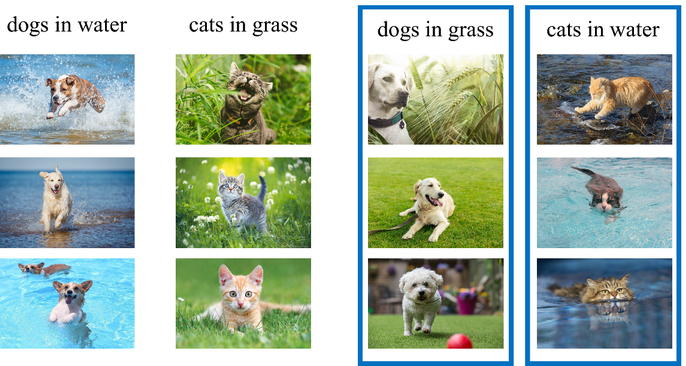
\includegraphics[width=0.8\textwidth]{images/covariate_shift.png}
	\caption{Esempio di covariate shift}
	\label{fig:covariate_shift}
\end{figure}
\subsection{Prior probability shift}
Il prior probability shift rappresenta il caso duale del covariate shift, focalizzato sul cambiamento della distribuzione della variabile target $y$, mentre la distribuzione condizionata delle feature data la classe rimane costante.
Formalmente:
\begin{definition}[Prior probability shift]
	Appare solamente nei problemi del tipo $Y \rightarrow X$ e si verifica nel caso in cui $P_{tr}(y) \neq P_{tst}(y) $ e $P_{tr}(x|y) = P_{tst}(x|y)$.
\end{definition}
Ad esempio, in un sistema di diagnostica medica per una specifica malattia infettiva, la distribuzione dei sintomi per i soggetti malati e sani rimane costante ($P(x|y)$ non cambia), ma la prevalenza complessiva della malattia nella popolazione $P(y)$ fluttua nel tempo (ad esempio, a causa di un'improvvisa epidemia o di una campagna vaccinale).
\subsection{Concept Shift (o Concept Drift)}
Il concept shift (o concept drift) si verifica quando cambia la relazione funzionale o semantica tra le feature di input e la variabile target, modificando di fatto la definizione stessa della classe da apprendere. Rappresenta la sfida più complessa, poiché i criteri decisionali appresi dal modello durante l'addestramento non sono più validi nell'ambiente operativo.
Formalmente:
\begin{definition}[Concept shift] Si verifica nel caso in cui:
	$$
		\begin{aligned} P_{tr}(y|x) \neq P_{tst}(y|x) \quad \text{e} \quad P_{tr}(x) = P_{tst}(x) & \quad (\text{nei problemi }X\rightarrow Y) \\ P_{tr}(x|y) \neq P_{tst}(x|y) \quad \text{e} \quad P_{tr}(y) = P_{tst}(y) & \quad (\text{nei problemi } Y \rightarrow X) \end{aligned}
	$$
\end{definition}
Ad esempio, nei sistemi di filtraggio dello spam o di rilevamento delle intrusioni di rete, gli utenti malintenzionati modificano attivamente le proprie strategie per eludere i filtri esistenti, cambiando la definizione di ciò che costituisce un'e-mail di spam o un attacco, lasciando però apparentemente inalterata la struttura generale del traffico dati.
\section{Cause del drift}
Si possono rilevare due principali cause del data drift:
\begin{itemize}
	\item \textbf{Sample Selection Bias}:
	Avviene quando il metodo di campionamento o di etichettatura dei dati di addestramento non è uniforme o casuale rispetto alla popolazione reale.
	\item \textbf{Ambienti Non Stazionari }: Molti contesti operativi sono intrinsecamente dinamici nel tempo e nello spazio. 
	In generale, gli ambienti sono dinamici e, talvolta, la difficoltà nel far corrispondere lo scenario di apprendimento all'utilizzo nel mondo reale è dovuta proprio a questi cambiamenti. Tali scenari rendono complesso valutare l'adeguatezza di uno specifico modello in presenza di variazioni ambientali, aumentando così la probabilità di shift.
	
\end{itemize}